\title[Causality]{Causality:\\ Course Logistics}
\author[Mooij \& Forr\'e]{\\[5mm]\large Joris Mooij \& Patrick Forr\'e\\
\url{j.m.mooij@uva.nl}, \url{p.d.forre@uva.nl}}
\institute[UvA]{
\begin{tikzpicture}
%  \node at (0,0) {\includegraphics[height=15mm]{amlab}};
  \node at (6,0) {\includegraphics[height=7mm]{uva_logo_en}};
%  \node[text width=4cm,text centered] at (0,1) {\small Institute for Computing\\ and Information Sciences};
%  \node[text width=4cm,text centered] at (7,1) {\small Informatics Institute};
\end{tikzpicture}
}
\date[2025-02-06]{\normalsize February 6, 2025}
\maketitle
\begin{frame}{Teachers}
  Lecturers:\\
  \scalebox{1.00}{\begin{tikzpicture}
      \node at (-4,0) {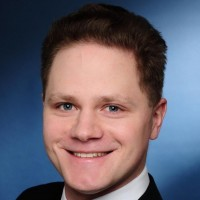
\includegraphics[height=2cm]{PatrickForre.jpg}};
      \node at (-4,-1.5) {Patrick Forr\'e};
      \node at (-4,-2) {\footnotesize \url{p.d.forre@uva.nl}};
      \node at (0,0) {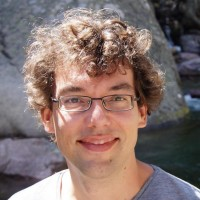
\includegraphics[height=2cm]{JorisMooij.jpg}};
      \node at (0,-1.5) {Joris Mooij};
      \node at (0,-2) {\url{j.m.mooij@uva.nl}};
  \end{tikzpicture}}

  \bigskip
  Teaching assistant:\\
  \begin{tikzpicture}
  %    \node at (-4,0) {
\includegraphics[height=2cm]{NoudDeKroon.jpg}};
  %    \node at (-4,-1.5) {Noud de Kroon};
  %    \node at (-4,-2) {\footnotesize \url{a.a.w.m.dekroon@uva.nl}};
      \node at (0,0) {
\includegraphics[height=2cm]{PhilipBoeken.jpg}};
      \node at (0,-1.5) {Philip Boeken};
      \node at (0,-2) {\footnotesize \url{p.a.boeken@uva.nl}};
  \end{tikzpicture}
\end{frame}

\begin{frame}{Aim of the course}
  Many questions in science and society are of a \emph{causal} nature. 
  \begin{itemize}
    \item How can we \emph{formalize} the notion of causality? 
    \item How to \emph{reason} about cause and effect mathematically? 
    \item How can we \emph{discover} causal relations from data? 
    \item How to \emph{predict} the consequences of actions? 
  \end{itemize}
This course will address all these questions, making use of the
mathematical frameworks of causal Bayesian networks and structural causal models.
\end{frame}

\begin{frame}{Target audience}
  This is a MasterMath course aimed at MSc.\ Mathematics students.

  \bigskip
  We also welcome:
  \begin{itemize}
    \item students from other MSc.\ programs (SFM, AI, econometrics, \dots)
    \item PhD students
  \end{itemize}
%  BUT: hard work may be required to compensate for mathematical deficits, in particular to acquire \textbf{passive understanding of measure theoric formulations}.
  
  \bigskip
  Prerequisites:
  \begin{enumerate}
    \item bachelor level probability theory\\
      {\tiny(e.g., G. Grimmett and D. Welsh, 'Probability - An introduction', 2nd edition)}
\item bachelor level measure theory\\
  {\tiny(e.g., R. Schilling, 'Measures, Integrals and Martingales' (2nd edition), Cambridge University Press, 2017)}
\item bachelor level statistics\\
  {\tiny(e.g., F. Bijma, M. Jonker, A. van der Vaart, 'An introduction to Mathematical Statistics', Amsterdam University Press, 2017)}
  \end{enumerate}
\end{frame}

\begin{frame}{Course materials}
  \begin{itemize}
    \item Course page on \url{elo.mastermath.nl} 
    \item Live lectures (will be video recorded)
    \item Lecture notes (Part I can be downloaded from ELO, Part II follows later)
    \item Weekly practice exercises
    \item Bi-weekly hand-in exercises
%    \item Video lectures from last year (as backup in case of illness etc.)
  \end{itemize}
\end{frame}

\begin{frame}{Timeline}
  Lectures are each Thursday, 14:00--16:45 at the VU.
  \begin{itemize}
    \item Weeks 6-12: Patrick teaches Part I (Markov kernels, Causal Bayesian Networks)
    \item Week 13-21: Joris teaches Part II (Structural Causal Models, Advanced Topics)
    \item Break in week 18 (May 1st)
    \item Exam on Thursday, June 19, 13:45--16:45
    \item Retake on Thursday, July 10, 13:45--16:45 
  \end{itemize}

  \bigskip
  \footnotesize\begin{tabular}{l|l}
    Weeks & Room \\
    \hline
    6--17       & NU 4A67 \\
    19--21      & NU 4A67 \\
    25 (Exam)   & HG 14A00 \\
    28 (Retake) & NU 4A67
  \end{tabular}
\end{frame}

\begin{frame}{Exercises, grading}
  \begin{itemize}
    \item Weekly exercise session with practice exercises
    \item Bi-weekly hand-in exercises that will be graded
  \end{itemize}

  \bigskip
  Final degree will consist of
  \begin{itemize}
    \item 15\% hand-in exercises
    \item 85\% final exam (or retake, if applicable)
    \item A student should get at least a 5.0 on the final exam or retake to pass
    \item The homework still counts as part of the grade after the retake
  \end{itemize}
\end{frame}

\begin{frame}{Questions?}
  Any questions?

\bigskip
\bigskip
\bigskip
  \centerline{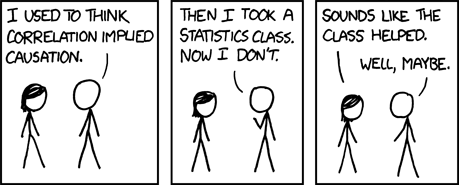
\includegraphics[width=0.7\textwidth]{correlation.png}}
\end{frame}
